\begin{figure}[H]
\centering
\def\axislength{.2}
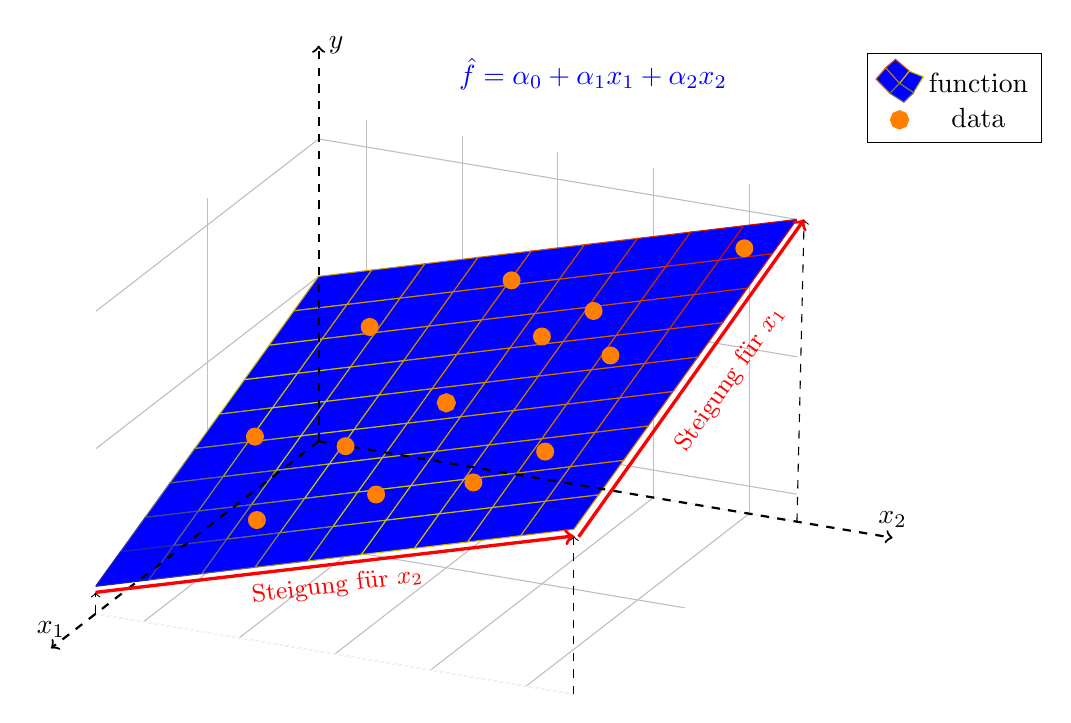
\begin{tikzpicture}
\pgfplotsset{
    axis line style={white},
  }
  \begin{axis}[scale=1.3,ticks=none, grid=major, legend style={at={(1.1,1.1)},anchor=north west} ]
    \coordinate (O) at (rel axis cs:0,1,0);
    \coordinate (x) at (rel axis cs:0,-\axislength,0);
    \coordinate (y) at (rel axis cs:1+\axislength,1,0);
    \coordinate (z) at (rel axis cs:0,1,1+\axislength);
    
    \coordinate (mx2b) at (rel axis cs:0,0,0.065);
    \coordinate (mx2e) at (rel axis cs:1,0,0.48);
     \coordinate (mx1e) at (rel axis cs:1.015,1,0.92);
    \coordinate (mx1b) at (rel axis cs:1.01,0,0.48);
    \coordinate (labelx1) at (rel axis cs:1,0.95,0.7);
    
    \coordinate (fst) at (rel axis cs:0,0,0);
    \coordinate (snd) at (rel axis cs:1,0,0);
    \coordinate (thd) at (rel axis cs:1,1,0);   
    
    \coordinate (f) at (rel axis cs:0.9,0.3,1.7);
    
    \coordinate (p1) at (rel axis cs:0.5,0.5,0.5);  
    \coordinate (p2) at (rel axis cs:0.23,0.23,0.22);
    \coordinate (p3) at (rel axis cs:0.71,0.71,0.72);
    
    \coordinate (p4) at (rel axis cs:0.2,0.8,0.5);  
    \coordinate (p5) at (rel axis cs:0.4,0.4,0.25);
    
    \coordinate (p6) at (rel axis cs:0.8,0.3,0.53);
    \coordinate (p7) at (rel axis cs:0.65,0.3,0.4);  
    
    \coordinate (p8) at (rel axis cs:0.45,0.9,0.65);
    
    \coordinate (p9) at (rel axis cs:0.35,0.37,0.4);
    \coordinate (p10) at (rel axis cs:0.1,0.5,0.3);  
   
    \coordinate (p11) at (rel axis cs:0.7,0.5,0.75);
    
    \coordinate (p12) at (rel axis cs:0.75,0.7,0.6);
    \coordinate (p13) at (rel axis cs:0.925,0.925,0.85);  
   
    \addplot3[surf, color=blue, samples=10] {x+y};
    \addlegendentry{function}
    \addplot3[mark=*,
			  only marks,
			  mark options={line width=0.1cm, color=orange,fill=orange}] coordinates{(0,0,0)};
    \addlegendentry{data}
  \end{axis}
  \draw[thick,dashed,->] (O) -- (x) node[above] {$\boldsymbol{x_1}$};
  \draw[thick,dashed,->] (O) -- (y) node[above] {$\boldsymbol{x_2}$};
  \draw[thick,dashed,->] (O) -- (z) node[right] {$\boldsymbol{y}$};
  
  \draw[dashed,->] (fst) -- (mx2b) node[above] {};
  \draw[dashed,->] (snd) -- (mx2e) node[right] {};
  \draw[dashed,->] (thd) -- (mx1e) node[right] {};
  
  \draw[red,very thick,->] (mx2b) -- (mx2e) node[rotate=7,below, midway] {\small Steigung für $x_2$};
  \draw[red,very thick,->] (mx1b) -- (mx1e) node[rotate=55,left] at (labelx1) {\small Steigung für $x_1$};
  
  \node[blue] at(f){$\boldsymbol{\hat{f} = \alpha_0 + \alpha_1 x_1 + \alpha_2 x_2}$};
  
  \draw[orange,thick,fill=orange] (p1) circle[radius=0.1cm];
  \draw[orange,thick,fill=orange] (p2) circle[radius=0.1cm];
  \draw[orange,thick,fill=orange] (p3) circle[radius=0.1cm];
  \draw[orange,thick,fill=orange] (p4) circle[radius=0.1cm];
  \draw[orange,thick,fill=orange] (p5) circle[radius=0.1cm];
  \draw[orange,thick,fill=orange] (p6) circle[radius=0.1cm];
  \draw[orange,thick,fill=orange] (p7) circle[radius=0.1cm];
  \draw[orange,thick,fill=orange] (p8) circle[radius=0.1cm];
  \draw[orange,thick,fill=orange] (p9) circle[radius=0.1cm];
  \draw[orange,thick,fill=orange] (p10) circle[radius=0.1cm];
  \draw[orange,thick,fill=orange] (p11) circle[radius=0.1cm];
  \draw[orange,thick,fill=orange] (p12) circle[radius=0.1cm];
  \draw[orange,thick,fill=orange] (p13) circle[radius=0.1cm];
  
\end{tikzpicture}
\caption[Grafische Darstellung der multiplen Regression]{Grafische Darstellung der multiplen Regression\protect\footnotemark}
\label{mr}
\end{figure}
\footnotetext{Eigene Darstellung}